\documentclass[10pt,twocolumn]{article}

% ---------------------------------------------------------------------------
% An idiomatic formally verified DER/X.690 encoding core in Rust (with
% structural X.509 parsing): a dual-layer proof architecture + honest envelope.
%
% Artifact / experience paper for the `der-verified` crate
% (https://github.com/ivmat/rs-verified-der, crates.io: der-verified).
%
% Self-contained: builds with two passes of pdflatex, no bibtex/biber needed.
% ---------------------------------------------------------------------------

\usepackage[utf8]{inputenc}
\usepackage[T1]{fontenc}
\usepackage{lmodern}
\usepackage{microtype}
\usepackage{booktabs}
\usepackage{array}
\usepackage{amsmath,amssymb}
\usepackage{listings}
\usepackage{xcolor}
\usepackage{tikz}
\usetikzlibrary{positioning}
\usepackage{url}
\usepackage[hidelinks]{hyperref}
\usepackage{enumitem}

\setlist{noitemsep,topsep=2pt}

\definecolor{codebg}{gray}{0.96}
\lstset{
  basicstyle=\ttfamily\footnotesize,
  breaklines=true,
  columns=fullflexible,
  backgroundcolor=\color{codebg},
  frame=none,
  xleftmargin=2pt,
  keepspaces=true,
  aboveskip=4pt,belowskip=4pt,
}

\newcommand{\code}[1]{\texttt{\small #1}}
\newcommand{\crate}{\code{der-verified}}

\title{\vspace{-2.5em}An Idiomatic Formally Verified DER/X.690 Encoding Core in
Rust (with Structural X.509 Parsing):\\
A Dual-Layer Proof Architecture and an Honest Proof Envelope}

\author{Ivo Matija\v{s}evi\'c\\
\small Independent researcher\\
\small \href{mailto:ivomatijasevic@gmail.com}{ivomatijasevic@gmail.com} \quad
\small \url{https://github.com/ivmat/rs-verified-der}}

\date{}

\begin{document}
\maketitle

\begin{abstract}
The DER encoding layer beneath X.509 is a recurring source of memory-safety
bugs and, more insidiously, \emph{parser differentials}---disagreements
between implementations about whether the same bytes are a valid certificate.
Unlike the higher X.509 profile, this layer has a small, checkable contract:
accept a byte string \emph{if and only if} it is the unique canonical DER
encoding, and never panic doing so. We report on \crate{}, an idiomatic Rust
DER/X.690 encoding core built so that its correctness evidence
\emph{re-runs from a fresh clone}. The crate combines two verification
lineages over the same source: a mandatory, exhaustive-but-bounded Kani/CBMC
floor of 171 proof harnesses across 26 modules---each harness proving its own
asserted property (safety, and per codec some of round-trip, minimality, or
rejection) over a stated bound---and an optional, additive set of six
Aeneas${\to}$Lean~4 ``lids'' that lift six codecs (three leaf codecs where an
$\forall$-length guarantee is most valuable and the functional model is
cleanest, plus the tag codec and, on the structural composition layer, the
TLV header/length pairing and the SEQUENCE child-walk---the latter the
crate's first $\forall$-length \emph{and} $\forall$-children, unbounded-loop
lid) to inputs of \emph{any} length, gated by a drift-detecting re-extraction
check.
We describe (i)~the dual-layer architecture and the build engineering that
lets a stable-toolchain Kani gate coexist with a nightly-pinned extraction
pipeline without duplicating source; (ii)~two API- and proof-structuring
techniques that make an idiomatic decoder BMC-tractable---a symbolic-length
discharge rule for modular stub proofs, and a two-tier strict/permissive
decode API that closes the trailing-byte differential surface at the crate's
top-level entry points; (iii)~a measured cost profile in which CBMC's
symbolic-execution \emph{formula construction}, not SAT solving, was the wall
on our hardest nested-container proof, and solver choice a modest,
harness-specific lever; and
(iv)~an ``honest proof envelope'' discipline---a first-class manifest of
bounds, assumptions, stubs, and explicit non-goals---that we position as a
concrete, author-side answer to recent critiques of ``verification theatre.''
We also document a silent Aeneas failure mode (extraction that ``succeeds'' by
degrading a function to a bodyless axiom) and its refactor fix. None of the
individual ingredients is new; the contribution is the specific, reproducible
combination on a real DER/X.509 target, reported honestly.
\end{abstract}

\section{Introduction}

A large fraction of TLS handshakes, code signatures, and PKI checks rest on
parsing X.509 certificates, which are serialized in DER---the Distinguished
Encoding Rules, a canonical subset of ASN.1's Basic Encoding Rules (X.690).
That encoding layer has a long, ugly track record: memory-safety bugs in C
parsers, and \emph{parser differentials}, where two implementations disagree on
whether a given byte string is a valid certificate. Differential-testing work
such as \emph{Frankencerts}~\cite{frankencerts} demonstrated how routinely
production stacks diverge---one library rejects bytes another accepts, one
normalizes a non-canonical length another treats as a distinct value---and such
disagreements are a recurring source of certificate-confusion and
validation-bypass bugs. Empirical studies of in-the-wild X.509
parsing~\cite{parseval} continue to find such divergence.

DER is, in principle, the friendly case. Every value has \emph{exactly one}
valid encoding, so a decoder has a crisp, checkable contract: accept a byte
string if and only if it is the unique canonical DER encoding, and never
panic. That contract is small enough to \emph{prove}, and proving it is a
real, if narrow, reduction of attack surface.

This paper is an experience report on \crate{}~\cite{repo}, a from-scratch
Rust DER/X.690 encoding core (published to crates.io) in which every public
codec carries machine-checkable evidence, and that evidence re-runs from a
fresh clone---the proofs are the product, not a badge. The crate is
\code{\#![forbid(unsafe\_code)]}, dependency-free, and allocation-free on its
decode paths. It is deliberately \emph{idiomatic} Rust rather than a
verification-DSL artifact: the same source that ships is the source that is
verified.

\paragraph{What is and is not new.}
We claim no new verification \emph{technique}. Kani/CBMC bounded model
checking~\cite{kani}, Aeneas/Charon functional translation of Rust to
Lean~4~\cite{aeneas}, and---as established practice in high-assurance
verification---layered assurance, explicit TCB/scope reporting, and deliberate
spec-scoping are all prior art. The nearest neighbour in the same domain, Verdict~\cite{verdict},
is a single-layer, Verus-verified end-to-end X.509 \emph{validator}. Our
contribution is instead an \emph{artifact}: a specific, reproducible
combination---an idiomatic Kani-verified Rust DER crate with optional
extraction-based unbounded lids, a drift gate tying the two together, and an
explicit ``what is \emph{not} proven'' discipline---reported with its costs
and its gotchas rather than only its successes. We believe the honest
combination is itself worth the record; recent work on ``verification
theatre''~\cite{theatre} argues, with thirteen concrete escapes from
formally verified crypto libraries, that the gap between what a project's
marketing claims and what its proofs actually cover is a live, systemic risk.
The proof envelope discipline in \S\ref{sec:envelope} is designed to make
that gap small and legible from the author's side.

\paragraph{Scope of the verified core.}
In scope (verified): the DER encoding layer---identifier (tag) and
definite-length fields, and the canonical content codecs \code{BOOLEAN},
\code{INTEGER} (both \code{i64} and arbitrary-magnitude), \code{NULL},
\code{OBJECT IDENTIFIER}, \code{BIT STRING}, \code{OCTET STRING},
\code{ENUMERATED}, the ASCII-restricted strings, \code{UTF8String},
\code{UTCTime}, \code{GeneralizedTime}, \code{SEQUENCE}, and \code{SET OF}
member ordering (\S11.6). The \code{x509\_*} modules parse RFC~5280 objects
(\code{AlgorithmIdentifier}, \code{SubjectPublicKeyInfo}, \code{Name},
\code{Validity}, \code{Extension}, \code{TBSCertificate}, \code{Certificate})
by composing the verified codecs, but interpret \emph{no} algorithm, key,
signature, or trust semantics. A separate \code{profile} module sits above
those parsers and is Kani-proven, but not Lean-lidded: it checks three
RFC~5280 \emph{cross-field} rules (signature-algorithm agreement,
extensions-imply-v3, and the UTCTime/GeneralizedTime year-2050 encoding
choice) as biconditionals over already-materialized field \emph{values}
rather than over DER bytes, so it carries Kani's assurance grade but not
L4's. Out of scope (and explicitly \emph{not}
proven): cryptography, path/trust validation, and the rest of the RFC~5280 profile.
This fence is not incidental---it is the crate's central honesty claim
(\S\ref{sec:scope},\S\ref{sec:envelope}). We stress up front that the claim is
\emph{per-codec and per-bound}: which property (round-trip, minimality, an
acceptance biconditional, or panic-freedom alone) is proven, and under what
bound, varies by module and is listed in the manifest; the \code{x509\_*}
modules carry structural panic-freedom evidence, not verified RFC~5280
semantics; and ``if and only if'' holds only where a named harness or Lean
theorem proves both directions for the implemented profile.

\section{The dual-layer architecture}
\label{sec:arch}

The verification stack has two lineages over the \emph{same} Rust source
(Figure~\ref{fig:arch}). We name them by assurance depth.

\begin{figure}[t]
\centering
\resizebox{\columnwidth}{!}{%
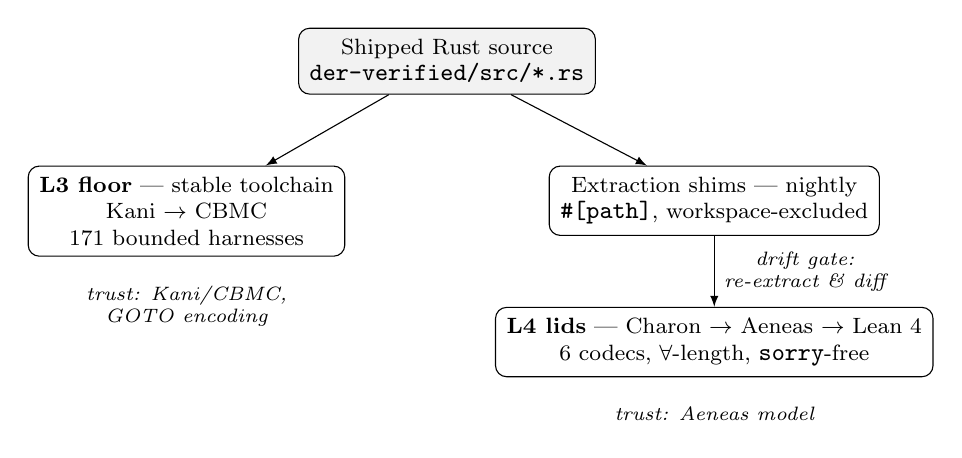
\begin{tikzpicture}[>=latex, font=\footnotesize,
  box/.style={draw, rounded corners, align=center, inner sep=4pt},
  note/.style={font=\scriptsize\itshape, align=center}]
\node[box, fill=black!5] (src) {Shipped Rust source\\\code{der-verified/src/*.rs}};
\node[box, below left=9mm and -6mm of src] (l3)
  {\textbf{L3 floor} --- stable toolchain\\Kani $\to$ CBMC\\171 bounded harnesses};
\node[box, below right=9mm and -6mm of src] (shim)
  {Extraction shims --- nightly\\\code{\#[path]}, workspace-excluded};
\node[box, below=9mm of shim] (l4)
  {\textbf{L4 lids} --- Charon $\to$ Aeneas $\to$ Lean~4\\6 codecs, $\forall$-length, \code{sorry}-free};
\draw[->] (src) -- (l3);
\draw[->] (src) -- (shim);
\draw[->] (shim) -- node[right, note] {drift gate:\\re-extract \& diff} (l4);
\node[note, below=2.5mm of l3] {trust: Kani/CBMC,\\GOTO encoding};
\node[note, below=2.5mm of l4] {trust: Aeneas model};
\end{tikzpicture}}
\caption{Two lineages over one source. The L3 stable Kani floor is mandatory;
the L4 nightly extraction lids are optional and additive, tied to the same bytes
by the drift gate. Each layer's trust boundary is labelled; the two are
complementary, not independent (both begin with the same Rust).}
\label{fig:arch}
\end{figure}

\paragraph{L3 --- the floor (mandatory, bounded).}
171 Kani proof harnesses across 26 modules. Kani compiles each
\code{\#[kani::proof]} to CBMC and discharges it as a bit-precise SAT/SMT
query. Every harness proves, by Kani's default checks, memory safety, absence
of panics, and absence of arithmetic overflow on its input domain, plus the
functional properties each harness asserts: decode/encode round-trip,
canonicality/minimality, and rejection of malformed or non-canonical
encodings. ``Bounded'' has a precise meaning here: each harness constructs a
fixed-size symbolic input (\code{kani::any()} byte arrays of a chosen length),
optionally narrowed by \code{kani::assume(\ldots)} preconditions, and unrolls
loops to a stated \code{\#[kani::unwind(N)]} depth (depths in use range 1--22,
most codecs at 16). The proof is therefore \emph{complete over that bounded
input domain and no larger}. Running the floor requires only \code{cargo} and
the Kani toolchain.

\paragraph{L4 --- the lids (optional, additive, unbounded).}
Bounded proofs leave a nagging question: what about inputs larger than the
bound? For six codecs---\code{length} (\S8.1.3), \code{big\_integer}
(\S8.3), \code{oid} (\S8.19), \code{tag} (\S8.1.2), \code{tlv} (the
tag/length header composition), and \code{sequence} (\S8.9/\S8.10, the
crate's first \emph{structural-composition} and first \emph{unbounded-loop}
lids)---the Rust is additionally translated,
Rust~$\to$~Charon~$\to$~Aeneas~$\to$~Lean~4, into a pure functional model, and
the corresponding properties are proven in Lean for inputs of \emph{any}
length (and, for \code{sequence}, any number of children), \code{sorry}-free
(Table~\ref{tab:l4}). The L4 layer lifts exactly the
codecs and composition points where an $\forall$-length guarantee is most
valuable and the functional model is cleanest. The \code{tag} lid was added
after (and specifically to reduce) the \code{tlv}/\code{sequence} lids'
own trust surface: both had originally treated \code{decode\_tag} as a
bodyless axiom (\code{tag\_decode\_total}, \code{tag\_decode\_used\_bounds})
because of the same depth-two-loop \code{return} shape \S\ref{sec:gotcha}
describes for \code{oid} defeated Aeneas extraction of a body; these were
crate-specific, hand-written characterizations of \code{decode\_tag}'s own
totality and consumption bound---not specifications of any Aeneas standard-
library primitive---asserted as axioms only because the extraction produced no
body to prove them against. Refactoring \code{tag} the same way and proving
its own lid discharged those four axiom instances, shrinking each of
\code{tlv}'s and \code{sequence}'s disclosed assumed-spec counts from seven to
six.

\begin{table}[t]
\centering
\footnotesize
\begin{tabular}{@{}lp{4.4cm}@{}}
\toprule
Codec & Unbounded property proven ($\forall$-length) \\
\midrule
\code{length} & every branch of \code{decode\_length}; round-trip canonicality (\code{decode\allowbreak\_accepts\allowbreak\_only\allowbreak\_canonical}) \\
\code{big\_integer} & minimality biconditional, validate side (\code{validate\allowbreak\_iff\allowbreak\_minimal}); encode round-trip (\code{encode\allowbreak\_minimal\allowbreak\_integer\allowbreak\_into\allowbreak\_roundtrip}) \\
\code{oid} & OID canonical-form biconditional, validate side (\code{validate\allowbreak\_iff\allowbreak\_canonical}) \\
\code{tag} & \code{decode\_tag}'s totality and consumption bound (\code{tag\allowbreak\_decode\allowbreak\_total}, \code{tag\allowbreak\_decode\allowbreak\_used\allowbreak\_bounds}) \\
\code{tlv} & \code{decode\_tlv}'s structural correctness and no-over-read (\code{decode\allowbreak\_tlv\allowbreak\_structure}) \\
\code{sequence} & \code{decode\_sequence}'s structural correctness, $\forall$-length \emph{and} $\forall$-children (\code{decode\allowbreak\_sequence\allowbreak\_structure}) \\
\bottomrule
\end{tabular}
\caption{The six L4 Aeneas${\to}$Lean~4 lids. All \code{sorry}-free; the full
axiom set each rests on---beyond Lean's standard \code{propext} /
\code{Classical.choice} / \code{Quot.sound}, the named Aeneas-Std spec axioms
and \code{bv\_decide}'s certificate axiom---is disclosed via
\code{\#print axioms} (\code{sorry}-free is not axiom-free).}
\label{tab:l4}
\end{table}

\paragraph{The property that ties the layers together.}
Two design choices make the two-layer claim sound rather than cosmetic.
First, L4 is \emph{guarded}: the driver script \code{lean/check\_lean.sh}
no-ops (exit 0) when the Aeneas/Lean toolchain is absent, so the full gate
still passes on the Kani floor alone on a machine without the heavy extraction
stack. The lids are additive assurance, never a build prerequisite---a
practical necessity if contributors and CI are not all to be forced to
provision a proof assistant. Second, and more important, each lid
\emph{re-extracts its model from the exact shipped \code{.rs} on every run}
and the gate \emph{fails closed on drift} between the regenerated extraction
and the committed Lean source. This closes the classic extraction-verification
trap in which the proved model silently diverges from the shipped code: the gate
mechanically ensures the committed Lean model is \emph{syntactically identical}
to what the pinned Aeneas/Charon pipeline regenerates from the \emph{current}
shipped \code{.rs} (the same source the L3 floor proves), not a stale
hand-transcribed snapshot. The \emph{semantic} correspondence between that model
and the shipped Rust remains trusted (the trust base, below); the gate closes
the source-drift hole, not the translation gap (and, per \S\ref{sec:gotcha}, not
a silent axiom-degradation hole). The lid additionally fails closed on any
\code{sorry} (checked mechanically for \code{sorryAx} / ``declaration uses
\code{sorry}''). Because that re-extraction/diff step is a minutes-long
milestone gate wired only into the full \code{check.sh}, a per-commit
\emph{tripwire} narrows that window: a committed content-hash state file over
the six lidded source files, checked by \code{check\_fast.sh}, fails closed if
any of them changed without a corresponding full Lean re-verification (or is
explicitly acknowledged as pending debt). This tripwire is only as reliable as
its invocation, though: \code{check\_fast.sh} runs on every commit solely via
the git \code{pre-commit} hook installed by \code{install\_hooks.sh}, which is
opt-in, and CI does not run \code{check\_fast.sh} at all---so a contributor who
has not installed the hook can still land drift on a branch or in CI. The
backstop is \code{check.sh}'s own \code{--strict} invocation of the
lid-staleness gate at the next full milestone run, which fails closed on any
undischarged drift regardless of whether the per-commit tripwire ever fired.

\paragraph{Trust base (both layers).}
Neither layer is trust-free, and we enumerate both boundaries rather than hide
them. \emph{L3} trusts Kani's Rust${\to}$GOTO encoding, CBMC and its underlying
SAT/SMT solver (the proofs are not independently certificate-checked), and the
fact that Kani's bundled toolchain is a different compiler instance than the
\code{stable} \code{rustc} that ships the crate. \emph{L4} additionally trusts
the Lean~4 kernel, the disclosed non-standard axioms (the Aeneas-Std spec axioms
and \code{bv\_decide}'s certificate axiom), and the \emph{Aeneas model} of the
Rust---the Charon/Aeneas translation is not itself formally verified against
\code{rustc} semantics (the standard Aeneas assurance boundary). Both layers
also assume the extract shims' features/\code{cfg}s match the shipping build.
The two layers are therefore \emph{complementary}, not semantically independent
cross-validation: both begin with the same Rust and rustc-derived machinery.

\paragraph{Reconciling two toolchains without copying source.}
\label{sec:shim}
A build-engineering tension threatens the single-source-of-truth property. The
main Kani gate must stay pinned to the \emph{stable} Rust channel; Charon (the
Rust-to-LLBC front-end driving Aeneas) requires its own pinned \emph{nightly}
(\code{nightly-2026-06-01}). Copying the extracted source would risk exactly
the drift the L4 gate exists to prevent; repointing the whole crate to nightly
would risk the Kani gate. We resolve this with one small \emph{shim crate per
extracted module} (\code{lean/extract/}, \code{lean/extract-bigint/},
\code{lean/extract-oid/}, \code{lean/extract-tag/}, \code{lean/extract-tlv/},
\code{lean/extract-sequence/}), each of which (1)~\code{\#[path]}-includes the
\emph{exact same} source file from \code{der-verified/src/} rather than
duplicating it, (2)~carries its own \code{rust-toolchain.toml} pinned to
Charon's nightly, and (3)~is \emph{excluded} from the root Cargo workspace, so
it never participates in the main \code{cargo build}/\code{test}/\code{kani}
invocations and cannot regress the stable Kani gate. The individual Cargo
mechanisms (per-directory toolchain pins, workspace \code{exclude},
\code{\#[path]} inclusion) are standard; combining them into a per-module shim
that isolates a nightly extraction step from a stable proof gate on one source
file is the reusable idiom. Together with the drift gate, the source-of-truth
link is closed: the same source bytes proven by Kani are the bytes extracted and
proven by Lean (the Aeneas translation step over those bytes remains trusted, as
above).

\section{Making an idiomatic decoder BMC-tractable}
\label{sec:tractable}

Two techniques were necessary to verify idiomatic (non-DSL) Rust with a
bounded model checker at this scale. Both are stated as general rules; the DER
setting is the instance.

\subsection{Symbolic-length discharge for modular stub proofs}
\label{sec:symlen}

Large compositions are proven \emph{modularly}: an already-verified inner
parser is replaced in an outer harness by a \code{\#[kani::stub]} carrying the
inner function's proven postcondition, so CBMC reasons only about the
composition glue. The crate uses seven such stub applications across four
harnesses, forming a DAG (\code{x509\_certificate} $\to$
\code{x509\_tbs\_certificate} $\to$ \{\code{x509\_name} $\to$ its RDN lemma,
\code{x509\_extension}, and---in one positive-construction witness harness
only---\code{x509\_validity}\}); each link is a real function separately
proven panic-free.

The subtle part is \emph{how} the stub's contract is discharged. A DER parser's
control flow is length-dependent: every length check reads
\code{input.len()}, and the composition invokes a stubbed sub-parser on
\emph{suffix slices} of many different lengths, not only the outer buffer's
full length. Discharging the stub's postcondition lemma only at one fixed
length therefore leaves the compositional argument \emph{unsound}: every shorter
call length relies on an undischarged contract instance, while the harness still
passes. The rule we adopted repo-wide is to discharge each stub's contract over
a \emph{symbolic} input length:
\begin{lstlisting}
let len = kani::any();
kani::assume(len <= buf.len());
// prove the postcondition of f(&buf[..len])
\end{lstlisting}
Symbolic length closes the previously omitted \emph{length-domain} obligation,
but it is only one part of a sound modular replacement. We state the rule for
the case that actually holds in this crate---the stubbed callees are
\emph{pure functions over an immutable input slice} whose entire observable
effect is their return value (an \code{Ok(used)} byte count or a rejection), no
mutation, no aliasing, no side channel. Under that restriction, and checked by
hand per stub (see also \S\ref{sec:limits}), the replacement is sound when:
(a)~the real callee is separately proven to satisfy its \emph{exact relational
contract}---not merely panic-freedom, but the full result postcondition the stub
asserts (e.g.\ \code{validate\_rdn}'s $2 \le \mathit{used} \le
\mathit{input.len()}$), including how many input bytes it consumes;
(b)~\emph{bound dominance}---the discharge harness's buffer bound covers every
suffix length the outer call sites can pass ($N_\mathit{lemma} \ge
N_\mathit{caller}$); a symbolic discharge over a too-small buffer has the same
shape and the same silent ``both versions verify'' failure; (c)~every
\code{kani::assume} precondition in the discharge harness is established at each
outer call site; and (d)~the stub is a genuinely over-approximating
nondeterministic stand-in (a \code{kani::any()} result constrained to that
contract), so its outcomes---value \emph{and} consumed-byte count---are a
superset of the real callee's. The per-edge mapping (which harness stubs which
sub-parser, and where each stubbed callee's own contract proof lives) is the
manifest's stub table; a fully mechanized linkage would use Kani function
contracts (below) so (a) is enforced rather than argued. The move from the old
fixed-length form to the symbolic one is a strict \emph{generalization} (it
widens the covered domain from the single length $N$ to $0..=N$ and subsumes the
old proof), and was empirically nearly free because the discharge buffers were
already fully symbolic; it made the crate's ``up to $N$ octets'' claims actually
true.

Kani's function-contracts feature (\code{-Z function-contracts},
\code{\#[kani::requires]}/\code{\#[kani::ensures]} with
\code{proof\_for\_contract} / \code{stub\_verified}) is the institutional
mechanism for exactly this ``discharge a contract, then substitute it'' pattern;
we used hand-written \code{-Z stubbing} stubs instead, but the same
fixed-vs-symbolic-length discharge gap can arise in a \code{proof\_for\_contract}
harness, so the bound-dominance rule is complementary to that feature rather than
a gap in it. We have not found the specific failure mode called out explicitly
in the mainstream Kani/CBMC documentation~\cite{kani}; it is easy to miss
precisely because both the fixed- and symbolic-length versions verify.

\subsection{A two-tier decode API closes the trailing-byte differential}
\label{sec:twotier}

X.690~\S8.1.1.1 fixes the shape of a DER encoding (identifier, length, contents
octets)---so a byte string that \emph{purports to be one complete value} is
well-formed only if it is exactly one such TLV with nothing after it. (This is a
property of the complete-object API contract, not a blanket rule that any
decoder input may contain only one TLV: recursive ASN.1 encodings are precisely
sequences of component encodings.) A recursive descent parser therefore
legitimately needs to decode ``one TLV, then whatever comes after'' at every
\emph{inner} level---an inner value naturally has a byte suffix belonging to the
next sibling. Collapsing these two needs into one function with an ambiguous
contract is exactly how
trailing-byte parser differentials arise. We split the API into two statically
distinct tiers:
\begin{itemize}
\item \code{decode\_tlv} / \code{decode\_sequence\_tlv}: non-strict, consume
  one TLV and \emph{permit} a trailing suffix; used \emph{only} to drive
  recursive parsing of inner values.
\item \code{decode\_tlv\_strict} / \code{decode\_sequence\_tlv\_strict}:
  strict, require the input to be exactly one TLV and return a distinct
  \code{TrailingData} error otherwise; used as the \emph{only} top-level entry
  points (\code{parse\_certificate} uses the strict form, so appended bytes are
  rejected at the outer \code{SEQUENCE}).
\end{itemize}
Each tier's boundary property is separately machine-checked, on a
\emph{bounded} domain: one harness (\code{decode\_tlv\_structure}) proves over a
symbolic buffer that an accepted TLV consumes exactly
$\mathit{header}+\mathit{declared\_length}$ bytes and never over-reads; another
(\code{strict\_rejects\_trailing}) proves the strict wrapper returns
\code{TrailingData} on a valid TLV followed by \emph{one} arbitrary trailing
byte. Rejection of longer trailing suffixes follows from the exact-consumption
harness plus the strict wrapper's remainder check, but that is a source-level
argument, not the harness statement. Two honest limits: the surface is closed
\emph{at the crate's top-level entry points} (\code{parse\_certificate} uses the
strict form), and the permissive \code{decode\_tlv} / \code{decode\_sequence\_tlv}
remain \code{pub}---so a downstream caller could still use the non-strict tier at
top level. The discipline is enforced by naming and convention for external
users, not by Rust's type or visibility system; making the permissive tier
non-public (or exposing a typed recursive-vs-complete distinction) would harden
it further. The underlying DER rule is old and the strict/lenient distinction is
parser folklore; packaging it as two independently \emph{proven} API tiers is
the transferable idiom, applicable to any recursive TLV-shaped format with the
same ``inner permissive, outer strict'' structure. It is philosophically close
to EverParse/LowParse's per-combinator non-malleability and exact-consumption
proofs~\cite{everparse}, but organized around a Rust API split rather than
combinator composition.

\section{What actually costs}
\label{sec:cost}

We measured the full Kani suite and report it honestly, because ``how
expensive is this to reproduce?'' is a first-order question for an artifact
whose whole pitch is re-runnability. Numbers below are point-in-time on the
stated hardware; we treat the \emph{tiers} as durable and the exact seconds as
indicative.

\paragraph{The wall is formula construction, not solving.}
\label{sec:wall}
The hardest harness proves that validating an X.509 \code{Name}---a
\code{SEQUENCE OF SET OF AttributeTypeAndValue}, doubly nested and
variable-count, with DER-mandated canonical \code{SET OF} ordering---never
panics. Proving this over fully symbolic bytes made CBMC re-derive the
pairwise padded-byte ordering comparison (\code{set\_of::cmp\_padded}) across
every partition of the input, inside a three-deep loop nest. Memory climbed past
\textbf{100~GB during symbolic execution}, \emph{before the SAT solver ran}.
Crucially, reducing the unwind depth and shrinking the input buffer---both
tested independently---\emph{barely moved it}. The dominant driver was the
loop-nest product of the ordering machinery, not the loop bound. We frame this
as an artifact observation and a diagnostic procedure rather than a general law:
for \emph{this} harness, formula generation dominated, so on a nested-container
BMC proof one should first measure which phase (formula construction versus
solving) dominates, and whether the unwind/buffer knobs actually move it,
\emph{before} assuming they will. If they do not, the fix is proof
restructuring, not more compute. The general phenomenon (nested-loop CBMC
formula blowup dominating memory) is documented BMC behaviour~\cite{cbmcpath};
the measured DER instance and the ``knobs don't help here---it's structural''
diagnosis are our contribution.

\paragraph{The fix is the standard modular move.}
Following \S\ref{sec:symlen}, the heavy inner layer \code{validate\_rdn}
(one \code{RelativeDistinguishedName}) is proven panic-free once at its natural
scale (${\sim}17$~GB), establishing a postcondition
($2 \le \mathit{used} \le \mathit{input.len()}$); the outer
\code{validate\_name} harness then stubs \code{validate\_rdn} with that
contract and reasons only about the \code{Name} glue, in ${\sim}510$~MB. Same
theorem, split from an intractable ${>}100$~GB monolith into two pieces at
commodity large-memory-workstation scale (the ${\sim}17$~GB piece still exceeds
a 16~GB laptop and runs on the reference box)---and the reason \code{-Z stubbing}
is required to reproduce the floor.

\paragraph{Per-module cost profile.}
Table~\ref{tab:cost} summarizes the tiers, measured on a deliberately modest
16~GB Apple-silicon laptop with \code{cargo-kani 0.67.0} / CBMC~6.8.0. Cost is
heavily right-skewed: the large majority of the 171 harnesses finish
sub-second to a few seconds; a moderate tier runs single-digit to tens of
seconds; a heavy tail is dominated by the \code{set\_of} \S11.6 padded
comparison re-derived over symbolic content; and two harnesses exceed a 16~GB
laptop and are documented as reference-CI (large-box) checks. We stress that
counts are inventory, not coverage, and that \emph{every} listed harness
verifies successfully---nothing in the table is a failure, only a cost.

\begin{table}[t]
\centering
\footnotesize
\resizebox{\columnwidth}{!}{%
\begin{tabular}{@{}p{3.5cm}rr@{}}
\toprule
Tier / representative harness & Time & Peak RSS \\
\midrule
Fast majority (\code{length}, \code{oid}, \code{boolean}, \ldots) & $<1$--few s & small \\
\code{restricted\_string} (26-harn.\ total) & ${\sim}21$ s & --- \\
\code{x509\_certificate} never-panics & ${\sim}50$ s & --- \\
\code{utf8\_string::roundtrip} & ${\sim}109$ s & --- \\
\code{set\_of::tag\_correctness} & ${\sim}256$ s & ${\sim}5$ GB \\
\code{x509\_name::validate\_rdn} & --- & ${\sim}17$ GB$^\dagger$ \\
\code{x509\_extension} never-panics & DNF$^{\dagger\ddagger}$ & large \\
\bottomrule
\end{tabular}}
\caption{Kani cost tiers, measured on a 16~GB Apple-silicon laptop (Kani 0.67.0
/ CBMC 6.8.0). Rows are individual harnesses except where marked ``total.''
$^\dagger$exceeds the 16~GB laptop's physical memory; runs on the 16-core /
29~GB Linux reference box (where the full floor is ${\sim}40$~min at ${\sim}20$~GB
peak). $^\ddagger$did not finish within a 5-minute per-harness budget on the
laptop.}
\label{tab:cost}
\end{table}

\paragraph{Solver choice is a modest, harness-specific lever.}
On the slowest single harness (\code{set\_of::tag\_correctness},
${\sim}256$~s on the default solver), we measured the CBMC back-ends:
\code{cadical} at ${\sim}220$~s (${\sim}14\%$ faster) but higher peak memory
(${\sim}6.6$~GB), and \code{kissat} which did \emph{not} finish within a
5-minute budget despite lower memory (${\sim}4.7$~GB). The effect is modest and
direction-inconsistent, matching the SAT-competition folklore that solver
performance is instance-dependent with no universal winner. We therefore pin
\emph{no} solver crate-wide and recommend measuring the specific slow harness
one is iterating on. Kani's supported backends are documented~\cite{kani};
we simply supply one concrete comparative data point.

\paragraph{Reproducibility.}
CI runs the LIGHT tier of \code{gates/tiers.txt}---the memory-tractable share
of the floor, gated against CI's own shard filters by
\code{gates/check\_tier\_parity.py} so the two cannot silently drift apart---on
every push (143 of the 171 harnesses, filtered by module across parallel
runners); the six HEAVY modules (\code{set\_of}, \code{sequence},
\code{x509\_extension}, \code{x509\_certificate}, \code{x509\_tbs\_certificate},
\code{x509\_name}) peak above a standard 7~GB hosted runner and are documented
as local-milestone checks. The most recently committed full-suite run
(\code{evidence/check-ba40709.log}, commit \code{ba40709}, 2026-08-07; 16-core
/ 29~GB Linux reference box, sequential---no \code{-j}, since parallel
harnesses multiply peak RSS---inside a 22~GB memory cgroup) verified all 171
harnesses \code{SUCCESSFUL}, 0 \code{FAILED}, in 53m37s wall, alongside a green
\code{cargo test} and a green L4 Lean pass (six lids, \code{sorry}-free) and
the strict lid-staleness gate in the same run.

\section{Scoping honestly}
\label{sec:scope}

\subsection{Every narrowing is a recorded decision, not a silent gap}

\crate{} is a \emph{strict, deliberately narrowed} profile of DER/X.509, not a
best-effort partial implementation, and the difference is made explicit.
Concrete narrowings---each an explicitly recorded design decision with its own
rationale and status in a decisions ledger, and cross-referenced from the
manifest's ``deliberate
deviations'' and ``what is NOT proven'' sections---include: capping
\code{INTEGER} at \code{i64} with a \emph{separate} \code{big\_integer} module
for arbitrary magnitude (keeping each module's proof domain simple and
independently boundable); rejecting BER's constructed/segmented \code{OCTET
STRING} form (simultaneously a scope narrowing \emph{and} a
parser-differential hardening); validating only \code{SET OF} member ordering
(\S11.6) while leaving general \code{SET} (\S10.3) out of scope; rejecting the
leap-second \code{SS=60} time value as a profile choice, reducing time
validation to single-field range checks rather than full calendar semantics.
Deliberate spec-scoping for tractable verification is standard practice
(seL4, CompCert, and---in this very domain---Verdict~\cite{verdict}, which
necessarily scopes to policy-specific validators). The discipline we emphasize
is procedural: narrow at named points, record each narrowing as an
individually documented decision with its rationale and status, and surface the
resulting boundary as an explicit list rather than an implicit gap a user must
discover the hard way.
It is the difference between ``we verified X'' and ``we verified exactly
\emph{this} profile of X, and here is precisely where the fence is and why.''

\subsection{The proof envelope as a first-class, gated artifact}
\label{sec:envelope}

The single most reusable output of the project is not any one proof but the
discipline around the claim. \crate{} publishes \code{PROOF\_MANIFEST.md} as a
dedicated, README-gated document---the mandatory first read---whose explicit
purpose is to stop the crate's own impressive-sounding numbers from being
over-read as completeness. Its opening line: \emph{``Counts are inventory, not
coverage \ldots{} describes how much verification exists, not a guarantee that
every reachable behaviour is covered.''} The manifest then makes the actual
claim precise and auditable via:
\begin{itemize}
\item a \textbf{toolchain-pins table} (the recorded \code{rustc} version plus a
  floating \code{stable}-channel configuration---so a future clone may select a
  different stable compiler---and the exact Kani/CBMC/Lean/Aeneas/Charon
  versions/revisions the claims were checked against, with the Aeneas/Charon
  revisions mechanically \emph{enforced} by the drift gate);
\item a \textbf{per-module inventory table} (harness count, \code{\#[kani::unwind]}
  range, and whether an L4 lid exists), so a reader sees which module has what
  depth of assurance rather than an aggregate count;
\item explicit disclosure that \textbf{136 \code{kani::assume} preconditions}
  narrow the proved domain, with the framing that the properties hold
  \emph{for inputs satisfying the assumptions} and inputs outside them are
  simply not claimed;
\item a \textbf{modular-proof stub table} (which harness stubs which
  sub-parser, and where each stub's own proof lives), so compositional
  soundness is auditable rather than asserted;
\item a dedicated \textbf{``what is NOT proven'' scope fence} (no cryptography,
  no full profile semantics, bounded except the six L4 codecs, the
  Aeneas-translation trust gap), stated as prominently as what \emph{is}
  proven.
\end{itemize}
Stating assumptions and TCB explicitly is best practice in formal methods; the
reusable template here is a single crate-level manifest, cross-linked as the
\emph{primary trust artifact}, with the ``counts are inventory'' framing and a
per-module bound/assumption/stub table. We position this deliberately against
Kobeissi's ``verification theatre''~\cite{theatre}, which studies the same
underlying \emph{verification boundary} problem---the interface between
machine-checked code and trusted-but-unverified code---and documents thirteen
bugs escaping formal verification in production crypto libraries, from an
\emph{external audit} angle. The manifest is the complementary, \emph{author-side}
move: make the boundary a first-class, gated document by design, so the gap
between claim and coverage is small and legible before an auditor has to find
it. Calling \crate{} ``a verified X.509 parser'' would be a lie; it is a
verified \emph{encoding} layer, and the manifest keeps that honest.

\section{A toolchain gotcha worth reporting}
\label{sec:gotcha}

Preparing idiomatic Rust for Aeneas extraction surfaced a silent, dangerous
failure mode. Aeneas's Lean~4 backend does not (yet) support a \code{return}
nested two loop-levels deep---the crate's original \code{validate\_oid} had a
\code{return Err(Truncated)} inside a \code{while} inside an outer loop. The
documented Aeneas limitation is ``returns inside nested loops \ldots{} are not
supported yet''~\cite{aeneas}; what is \emph{not} documented is the
\emph{consequence}. Rather than erroring, extraction ``succeeds'' by silently
degrading the function to a \textbf{bodyless \code{axiom}}. A bodyless axiom is
unconstrained by the function's implementation, so it loses all correspondence
to the Rust---any lid ``proving'' a property about it says nothing about the
shipped code---yet the pipeline reports success. A contributor could ship a
``verified'' lid that is actually an unconstrained axiom without noticing,
unless they specifically inspect the generated Lean for \code{axiom}
declarations where a real definition was expected.

The fix was a source refactor: rewrite \code{validate\_oid} as a \emph{single
loop} with an explicit \code{at\_subid\_start} state variable, so every early
\code{return} sits at loop-depth~1. The refactor was \emph{regression-checked}
rather than assumed safe---the crate's five \code{oid} Kani harnesses and its 320
tests pass against it---which is bounded, example-based regression evidence,
\emph{not} a full behavioural-equivalence proof between the two implementations.
The refactored \code{oid} harnesses are also inexpensive today (${\sim}0.04$~s
per the cost note). The general recipe
(single loop + explicit state, keeping early returns at depth~1) is a reusable
pattern for Rust being prepared for Aeneas extraction, since early returns
inside nested loops are a common Rust parser idiom. We reported the silent-axiom
behaviour upstream (Aeneas issue \#1221~\cite{aeneasissue}); it is distinct
both from the documented general limitation and from the closest pre-existing
report, issue \#1206, which is a \emph{hard-error} failure mode (a \code{for}
loop with conditional \code{break}) rather than silent degradation. Note that
the crate's own L4 gate does \emph{not} fully catch this: the \code{sorry} check
does not fire on a bodyless axiom, and the drift gate only compares against the
\emph{committed} Lean, so a regenerate-and-commit workflow could launder a
degraded axiom in. Closing it properly needs a mechanical \emph{expected-definition}
gate---fail unless each lid's target function is emitted as a body-bearing
definition (equivalently, an allowlist for the extracted axioms/constants).
Until then we grep extracted Lean for unexpected \code{axiom} declarations as a
defensive check; we flag this residual hole candidly rather than imply the gate
already closes it.

\section{Related work}
\label{sec:related}

\paragraph{Verified X.509 in the same domain.}
Verdict~\cite{verdict} is the closest published prior art: an end-to-end,
Verus-verified Rust X.509 \emph{validator} with customizable, first-order-logic
validation policies and a proof-producing compiler, evaluated on over ten
million real certificates. It is single-layer (deductive verification, no BMC
floor and no extraction lids), targets the full validation problem
(parsing, path building, path validation), and verifies the Rust source
directly---so it has no extraction step and no drift surface to gate. Our
target is narrower and lower---the encoding brick---but the artifact is a
different \emph{architecture}: an idiomatic bounded floor plus optional
unbounded extraction lids over the same source. A recent
Rust${\to}$Charon${\to}$Lean pipeline with AI-prover assistance~\cite{ailpipeline},
applied to zero-knowledge-proof code, shares our toolchain family but is a
sequential pipeline, not a BMC-floor-plus-lid dual gate with drift detection.

\paragraph{Unverified Rust DER/X.509 crates.}
The incumbent Rust ecosystem---RustCrypto's \code{der} (which underpins
\code{x509-cert}) and \code{rasn}---is widely used but not formally verified.
We built a from-scratch idiomatic crate rather than retrofit proofs onto one of
these because a Kani/Aeneas-friendly proof surface (bounded symbolic buffers,
stubbable seams, single-loop functions amenable to extraction) is far easier to
design in than to retrofit onto code written without verification in mind; the
cost is reimplementing the encoding layer, and the benefit is that the shipped
code and the verified code are identical by construction.

\paragraph{Parser differentials.}
Frankencerts~\cite{frankencerts} and subsequent in-the-wild studies of X.509
parsing~\cite{parseval} motivate the problem class: the trailing-byte surface
that \S\ref{sec:twotier} addresses at the crate's top-level entry points, and
the malformed/non-canonical-encoding class the per-codec proofs reject.
EverParse/LowParse~\cite{everparse} provides verified parser combinators with
non-malleability and exact-consumption guarantees---philosophically close to
``prove each boundary property''---organized around combinator composition
rather than an idiomatic Rust API.

\paragraph{Verification honesty.}
Kobeissi's ``verification theatre''~\cite{theatre} is the most direct context
for \S\ref{sec:envelope}: it defines the verification boundary as the
structural failure pattern and argues, from an external-audit stance, that
overselling verification completeness is a live risk. The proof-envelope
manifest is the author-side counterpart. Stating TCB and scope explicitly is
long-established practice in high-assurance formal methods; our contribution is
a concrete, reusable crate-level template with mechanical drift enforcement.

\paragraph{BMC cost.}
The nested-loop CBMC formula-construction blowup we measure
(\S\ref{sec:wall}) is a documented characteristic of BMC
tools~\cite{cbmcpath,spaceefficientbmc}; our contribution is a concrete,
root-caused instance on
a real DER/X.509 target and the diagnostic that unwind/buffer tuning does not
move a structurally dominated cost.

\section{Limitations and threats to validity}
\label{sec:limits}

We collect the caveats stated throughout, since an experience paper's value
depends on them being legible in one place.

\emph{Assurance scope.} The L3 floor is \emph{bounded}: properties hold over
fixed-size symbolic buffers, under 136 disclosed \code{kani::assume}
preconditions, up to stated unwind depths; inputs outside those domains are not
claimed. Only six codecs have $\forall$-length L4 lids (and, for \code{sequence}
alone, an additional $\forall$-children lift over the same lid); every other
codec is Kani-bounded only. Even among the six, the lid's reach differs by
codec (\S\ref{sec:envelope}, PROOF\_MANIFEST.md \S6.2): \code{length},
\code{big\_integer} and \code{oid} carry unbounded canonicality/minimality
theorems (\code{decode\_accepts\_only\_canonical}, \code{validate\_iff\_minimal},
\code{validate\_iff\_canonical}), while \code{tag}, \code{tlv} and
\code{sequence} lift only structural totality/correctness---their rejection
classification (and, for \code{big\_integer}, the classification of specific
malformed shapes beyond the minimality biconditional) remains Kani-bounded.
The correctness of the
harness \emph{assertions} and the stub \emph{contracts} is itself a manual
modelling step; a wrong assertion proves the wrong thing. The modular proofs
rest on the refinement obligation of \S\ref{sec:symlen} (bound dominance,
precondition discharge, over-approximating stubs), checked by hand per stub, not
by a machine-checked meta-theorem.

\emph{Trust base.} L3 trusts Kani/CBMC (and its SAT/SMT solver, not certificate-
checked) and the Rust${\to}$GOTO encoding; L4 additionally trusts the Lean~4
kernel, the disclosed axioms, and the Charon/Aeneas translation against
\code{rustc} semantics. Both layers begin with the same source and rustc-derived
machinery, so they are complementary, not independent. \code{sorry}-free is not
axiom-free: the L4 proofs rest on named Aeneas-Std spec axioms and
\code{bv\_decide}'s certificate axiom (disclosed via \code{\#print axioms}). The
extract shims' features/\code{cfg}s are assumed to match the shipping build.
Moreover the L4 gate does \emph{not} mechanically exclude extraction that
degrades a function to a bodyless axiom (\S\ref{sec:gotcha}): the \code{sorry}
check does not fire on it and the drift gate compares only against the committed
Lean, so until an expected-definition gate exists this is guarded by a defensive
grep, not a fail-closed check.

\emph{Reproducibility and measurement.} The default gate conditionally
\emph{skips} L4 when the extraction toolchain is absent; a full-evidence run
must provision it. The Rust side is a \emph{floating} stable channel, so a
future clone may compile with a different \code{rustc}. All performance numbers
are point-in-time on the two stated machines and move with tool versions.

\emph{Behavioural claims.} The OID refactor (\S\ref{sec:gotcha}) is
regression-checked, not proven equivalent. The trailing-byte surface is closed
for the crate's own top-level entry points; the permissive tier remains public.
Regression tests, bounded proofs, and unbounded lids are three distinct grades
of evidence, and the manifest---not any aggregate count---is the actual claim.

\section{Conclusion}

You cannot (yet) formally verify ``X.509 is safe.'' But you can carve off the
encoding layer---the part with a crisp canonical-form contract and a bad CVE
history---and prove that brick does not panic and accepts only canonical
bytes, with evidence anyone can re-run from a fresh clone. \crate{} does this
with a mandatory bounded Kani floor and optional unbounded Aeneas${\to}$Lean
lids over the same idiomatic source, tied together by a drift-detecting gate,
and reported through a first-class honest proof envelope. None of the
ingredients is individually new; the reproducible combination, its measured
costs, and its gotchas---reported honestly rather than only in their best
light---are the artifact. It is also a template for doing the same to the
layers above.

\paragraph{Availability.}
\crate{} is on crates.io and at \url{https://github.com/ivmat/rs-verified-der}.
From a fresh clone, \code{./check.sh} reproduces the L3 floor (171 Kani
harnesses) and the 320 tests; it additionally re-extracts and checks the six
Aeneas${\to}$Lean lids \emph{when} the pinned extraction toolchain is present,
and otherwise skips them and still passes on the floor (\S\ref{sec:arch}). A
full-evidence reproduction (floor + lids + the honest proof envelope) therefore
requires provisioning that toolchain, as the README documents.

\begin{thebibliography}{99}
\footnotesize

\bibitem{repo}
I.~Matija\v{s}evi\'c.
\emph{der-verified: a formally verified DER/X.690 encoding core in Rust}.
crates.io / \url{https://github.com/ivmat/rs-verified-der}, 2026.

\bibitem{verdict}
Z.~Lin, M.~McLoughlin, P.~Singh, R.~Brennan-Jones, P.~Hitchcox, J.~Gancher,
and B.~Parno.
\emph{Towards Practical, End-to-End Formally Verified X.509 Certificate
Validators with Verdict}.
In \emph{34th USENIX Security Symposium}, 2025.
\url{https://www.usenix.org/conference/usenixsecurity25/presentation/lin-zhengyao}.

\bibitem{everparse}
T.~Ramananandro, A.~Delignat-Lavaud, C.~Fournet, N.~Swamy, T.~Chajed,
N.~Kobeissi, and J.~Protzenko.
\emph{EverParse: Verified Secure Zero-Copy Parsers for Authenticated Message
Formats}.
In \emph{28th USENIX Security Symposium}, 2019. (LowParse is the underlying
combinator library.) \url{https://project-everest.github.io/everparse/}.

\bibitem{frankencerts}
C.~Brubaker, S.~Jana, B.~Ray, S.~Khurshid, and V.~Shmatikov.
\emph{Using Frankencerts for Automated Adversarial Testing of Certificate
Validation in SSL/TLS Implementations}.
In \emph{IEEE Symposium on Security and Privacy}, 2014.

\bibitem{parseval}
S.~Tatschner, S.~N.~Peters, M.~P.~Heinl, T.~Specht, and T.~Newe.
\emph{ParsEval: Evaluation of Parsing Behavior using Real-world
Out-in-the-wild X.509 Certificates}.
In \emph{Proc.\ 19th Int.\ Conf.\ on Availability, Reliability and Security
(ARES)}, 2024. \url{https://arxiv.org/abs/2405.18993}.

\bibitem{ailpipeline}
N.~Klaus, J.~Conejero, and P.~Tolmach.
\emph{A Rust-to-Lean Verification Pipeline with AI Provers: An Experience
Report}.
AIMACS workshop at CAV, 2026. arXiv:2605.30106.
\url{https://arxiv.org/abs/2605.30106}.

\bibitem{theatre}
N.~Kobeissi.
\emph{Verification Theatre: False Assurance in Formally Verified Cryptographic
Libraries}.
IACR Cryptology ePrint Archive, Report 2026/192, 2026.
\url{https://eprint.iacr.org/2026/192}.

\bibitem{kani}
R.~Delmas, Z.~Hassan, Q.~Hu, R.~Kumar, F.~R.~Monteiro, T.~Nguyen, A.~Palacios,
C.~Val, M.~Tautschnig, J.~Adam, D.~Schwartz-Narbonne, and C.~Zech.
\emph{Kani: A Model Checker for Rust}.
In \emph{39th IEEE/ACM Int.\ Conf.\ on Automated Software Engineering (ASE),
Industry Showcase}, 2026. arXiv:2607.01504. Tool docs:
\url{https://model-checking.github.io/kani/}.

\bibitem{aeneas}
S.~Ho and J.~Protzenko.
\emph{Aeneas: Rust Verification by Functional Translation}.
In \emph{Proc.\ ACM Program.\ Lang.\ (ICFP)}, 2022. (Charon is the companion
Rust-to-LLBC front end.) \url{https://github.com/AeneasVerif/aeneas}.

\bibitem{aeneasissue}
Aeneas issue \#1221: silent degradation to a bodyless axiom on a \code{return}
nested two loop-levels deep (reported).
\url{https://github.com/AeneasVerif/aeneas/issues/1221}.

\bibitem{cbmcpath}
K.~Khazem and M.~Tautschnig.
\emph{CBMC Path: A Symbolic Execution Retrofit of the C Bounded Model Checker
(Competition Contribution)}.
In \emph{TACAS} (LNCS 11429), Springer, 2019.

\bibitem{spaceefficientbmc}
J.~Katz, Z.~Hanna, and N.~Dershowitz.
\emph{Space-Efficient Bounded Model Checking}.
arXiv:0710.4629, 2007, on BMC memory scaling from loop unrolling.

\end{thebibliography}

\end{document}
